\documentclass[a4paper,12pt]{article}
\usepackage{CJK}
\usepackage{graphicx}
\begin{document}

\begin{CJK}{UTF8}{gkai}
%\begin{CJK}{UTF8}{gbsn}
\section{密码电路故障攻击理论与技术}
\subsection{故障攻击的理论基础:包括攻击原理、基本假设、模型、方法和评价标准。此外,还将阐述一些常用的DFA和其他一些safe error的故障分析方法}
\subsubsection{故障分析的攻击原理和基本攻击方法,包括DFA和IFA,FSA等}

电子设备在运行时会受到各种各样自然的或是人为的干扰,在某些极端条件下设备停止工作或是输出不正确的结果。传统密码分析方法利用密码算法结构和一定明密文对来研究密码安全性,不同与此,故障攻击利用了设备在故障时的不正确结果中隐含的信息来辅助分析。故障攻击主要分为故障注入和故障分析两部分。故障注入主要研究密码设备在受到电压时钟毛刺,激光等干扰时的发生故障的模式;故障分析利用特定的故障输出作为辅助信息来完成密码分析,推导秘密信息。

最早的故障是偶然发生的,放射性元素衰变产生的带电粒子使得芯片出现了故障。之后为了提高芯片的稳定性和可靠性特别当芯片被用于外太空等极端环境下时,研究人员模拟和实验了大量不同的故障环境和对芯片的影响,这阶段研究的主要目的是研制高可靠性设备。

首个利用故障输出来推导密码算法的工作是由*Bellcore*等人在1997年提出的。该方法成功利用一对正确和错误密文对得出使用中国剩余定理实现的RSA算法的私钥。紧随其后故障分析的思想被Biham和Shamir等人用于分组密码DES的分析并提出了对几乎所有分组密码都有效的差分故障攻击。之后研究人员提出了大量的针对各种不同密码算法的故障分析和防护方案,使得故障分析成为一个极为活跃的研究领域。由于故障攻击可以在实际时间内成功攻击密码设备这也导致了对各种专用的故障注入设备的实验和开发。

在现行的软硬件架构和实现中故障注入可以影响程序的执行指令同时也可以影响程序的运算的中间值,对密码算法的故障分析主要集中于影响密码运算中间值的故障类型的分析。影响程序执行指令故障注入可以被用于跳过认证,修改程序流程等多种目的,但是在本章节中我们不考虑这种情况。

\subsubsection{故障模型分类和介绍}

故障模型是对设备在故障注入时产生的影响的抽象描述。故障模型要具有通用性,这样不同的密码算法不同的实现方式都可以通过故障模型加以描述同时这也提供一种便利的叙述背景和比较基准;故障模型也要具有可实现性,故障模型必须是实际的故障注入实验中可以重现的并且这种实现可以基于不同的软硬件设备和不同故障注入手段。

现在的分组密码大部分是迭代式的结构,算法包括多轮大致相同的轮函数,轮函数由几个操作构成,故障注入一般影响某个特定轮的特定操作的中间值或是某几个特定轮中的某个中间值,该中间值的长度一般为分组密码明文长度。在公钥等密码算法中,受影响的中间值一般可以限定为在执行某个操作或是某一组操作时。

一些为大部分研究者所使用和认可的故障模型有单比特故障模型,单字节故障模型。单字节模型,密码算法的中间值的某一比特位的值发生改变,受影响的比特的位置在目标中间值中是随机且均匀分布的,该比特位在受到故障注入影响后随机的变为0或1。单字节故障模型,目标中间值的某一个字节发生改变,受影响的字节的位置在中间值中是随机且均匀分布的,该字节的故障值是随机并且均匀分布的,即故障值为0~255中的任何一个的概率为1/256。

在不同的分析场景下还有一些不同的故障模型,如在safe  error的分析中,一般会假设受影响的比特、字节等的故障值为某一特定值。在轻量级分组密码的分析中,由于它们一般采用比较小(如3$\times$3,4$\times$4)的S盒,研究人员也会采用随机单S盒的故障模型。

随着故障攻击研究的深入,研究人员也在探讨各种新的故障模型,如故障位置或是故障值非均匀分布的故障,多字节的故障模型和更为通用的有偏差非特定型故障模型。

\subsubsection{故障攻击的评价指标,包括所用故障模型,故障数,攻击轮数,攻击的时间复杂度等。}
完整的故障攻击由故障注入和故障分析组成,对故障攻击的评价也分别对这两方面有不同的方式。

对于故障注入技术主要可从注入的时间和位置精度,注入后发生故障的可重复性,故障所能影响的芯片的类型或是其上的元件的类型,完成注入所需要的设备的成本和所需要的人员的技能等方面来加以评价。各种不同的故障注入方法各有自身的优缺点,可根据实际的成本和需求来选择相应的注入技术,这部分内容将在故障注入技术一节中进行较为详细的介绍。

故障分析的评价指标包括所用的故障模型,如前一节所述存在多种限制条件不同的故障模型,恢复密钥所需要的故障数,对于迭代式分组密码要考虑故障需要注入的轮数,和攻击所需要的时间复杂度。分析所采用的故障模型用通用,就可以越广泛的被用于各种故障注入生成的故障密文,效果也就越好。恢复密钥所需要的故障数越少越好,在故障注入结果产生的故障类型有多样性时,所需要的列举的情况是与故障数的指数成正比的。一种针对故障攻击的防护是,重算加密部分的最后几轮,比较两次计算的结果,为了实现的高效,往往会希望重算的轮数越少越好,故障分析能利用更早轮数的故障注入就能更好的攻击相应算法。例如,Bellcore实验室最先提出的针对RSA-CRT的攻击之需要在两个计算分支的任一位置出错,且只需要一个故障密文即可,因此是非常有效的攻击方式。

\subsection{先进分析方法:包括一些当前研究热点,如故障和功耗攻击结合的分析方法}
\subsubsection{故障和传统密码学分析方法的结合}

传统密码分析方法研究算法的数学结构,利用算法自身结构和采用的部件的弱点来进行分析。现有的比较有效的传统密码分析方法有差分分析,线性分析,不可能差分分析,积分攻击等。随着针对故障攻击的防护在密码电路中的广泛使用,故障的注入也越来越困难,产生的故障也越来越难以简单的加以利用,将故障分析与传统密码学分析方法结合也越来越引起研究者的注意。研究者将故障与不可能差分,中间相遇,线性分析等结合在不同方面对故障分析的能力进行了拓展。下面介绍代数攻击与旁路攻击的结合。

代数攻击的基本思想是将加密过程看做一个代数方程,密码的密钥和算法执行过程的中间值都作为该系统的未知参数。然后选择明密文对并将相应取值代入方程中可以获得一个代数方程组。最后求解方程组并获得密钥的取值。代数分析通常用在密码执行流程可以用比较简单的代数方程描述的算法,如AES和一些基于AES修改的密码。代数分析的复杂度在于其变量数和次数都较高,求解相应的代数方程的复杂度是NP完全的,无法在有效的时间内得到正确的解。故障攻击采用的故障模型和故障密文实际上为密码分析提供了额外的信息,这些都可以作为额外的变量和方程添加到原有方程组中,进而简化方程组的求解,从而恢复密钥。

LED是一个轻量级的分组密码,在CHES2011上由etal等人提出,在算法的设计上借鉴了AES。LED的分组长度为64比特,密钥长度可以为64比特或128比特,分别被记为LED-64和LED-128。对LED-64算法执行32轮,对LED-64算法执行48轮。算法的64比特中间状态都被划分为16个4比特分组并且类似AES放入到4$\times$4的矩阵中。每个四比特分组都被认为是有限域$\mathbb{F}_{16}\cong \mathbb{F}_{2}[x]/\langle x^{4}+x+1 \rangle$上的元素。

LED算法没有密钥生成算法,对于64比特密钥主密钥直接被用作白化密钥和轮密钥,轮密钥每隔四轮使用一次;对于128比特密钥主密钥被划分为两个64比特部分,在需要使用密钥时两部分密钥交替使用。密钥直接与算法的状态进行按位异或操作。算法轮函数类似AES,包括异或常数,S-box替换,行移位,列置换,每一个操作都可以用代数方程来加以表示,具体内容可参考。同时可根据故障模型和故障密文列出相应的方程。最终作者可以用包含有6336个未知变量的6208个多项式来表示加密过程,同时用包含有192个未知变量的48个方程来表示故障传播过程。将明文,密文,故障密文代入上述方程组可以分别消去128和64个位置变量。作者在有8个3.5GHz的CPU和50G内存的工作站上使用Minisat 2.2和CryptoMiniSat 2.9.4这两个SAT求解器来解生成的方程,实验结果表明仅使用一组正确错误密文对可以在20小时左右恢复。在代入故障密文时,作者采用计算机代数系统ApCoCoA来对生成的等式化简,然后再通过SAT求解器来求解,实验结果表明上述措施缩短了求解时间,采用单线程是平均求解时间为10小时。

\subsubsection{故障分析和功耗等旁路分析方法的结合}
故障攻击作为旁路攻击的一种,可以很方便的与其他旁路攻击方法如SPA,DPA,CPA等进行结合。在故障注入阶段,可采集电路的功耗或电磁辐射曲线通过SPA的方法观察并确定各个时间段电路进行的操作,从而提高故障注入的时间精度。在故障分析阶段同样可以结合故障与功耗或电磁辐射分析简化分析复杂度或是攻击带有一定防护能力的电路。本节攻击AES算法,该算法在实现时考虑了故障和功耗的防护,但是本节中描述的攻击显示只是简单的组合这两种防护并不足以抵御故障与功耗相结合的攻击方法。

目标算法针对故障攻击的防护是根据某一轮的中间结果重新计算密文并与正常加密运算的结果比较,如果相等则输入密文,否则芯片停止运行并丢弃相应密文。针对功耗分析的防护方案是采用高阶掩码。作者的故障模型假设故障发生在倒数第二轮的子密钥生成处,故障为可以为多字节故障但是要求有很高的可重现率。在正常加密和有故障注入时采集相应的功耗曲线共N组,记为$(C^{1},\Omega^{1}),\cdots,(C^{N},\Omega^{N})$。根据故障防护方案可知,在比较两次计算的密文时未加任何掩码,因此可以假设曲线上某一点处的功耗与故障密文相应字节的汉明重量存在相关性,记为$\Omega^{i}(t_{i})=\phi(C^{'i})+Noise$,其中C'为故障密文,Noise为噪声。对于故障密文的每个字节$j$,给出一组猜测值$(e_{9},e_{10},k})$并计算相关系数$\pho_{e_{9},e_{10},k}$。相关系数的计算方法如下,首先对于每个$C^{i}$,计算预测值$pred_{i}=HW(SubByte(SubByte^{-1}(C^{i}_{j}\oplus k)\oplus e_{9})\oplus k\oplus e_{10})$,然后计算预测值与功耗曲线上相关点的Peason相关系数$\pho_{e_{9},e_{10},k}=\pho(\{pred_{i}\}_{1\le i\ge N},\{\Omega^{i}[t_{i}]\}_{1\le i\ge N})$。找出使得相关性最大的故障和子密钥猜测值,如果相关系数超过某一阈值,可认为猜测的子密钥是正确的。综合每个字节的密钥猜测值就可以获得最后一轮轮密钥。

算法的成功率取决于旁路信号中噪音的大小,故障注入的可重复率和明文的数量。仿真结果表明达到90\%的成功率所需要的铭文书相对于噪音的标准差和故障的可重复率都是以指数的形式进行增长。但是在噪声达到实际强度并且故障的重现率只有约40\%时仍然可以使用不超过4000条曲线恢复最后一轮子密钥。

\subsubsection{故障攻击在未知但可区分的故障模型下的应用}
\subsection{各类密码结构/算法的故障分析方法:针对常用的对称密码和非对称密码,给出其结构弱点和故障攻击分析方式}
\subsection{DES故障攻击}
1996年,Biham和Shamir第一次提出了对DES的差分故障攻击(DFA),之后又有一些文章对此进行了扩展和改进,本节首先简要介绍DES算法,然后引入针对DES的后两轮原始故障攻击、中间轮故障攻击及基于内部碰撞的前几轮故障攻击。
\subsubsection{DES算法}
DES为64位的16轮Feistel结构(见图\ref{des_feistel}),每一轮的变换为$F_{K_r(L,R)=(R,L \oplus f_{K_r}(R))}$,其中L,R分别表示数据的左右部分,f是以48位密钥$K_r$为参数的32位输入到32位输出的映射函数(见图\ref{des_f_function})
\begin{figure}
\centering
\caption{Des feistel结构}
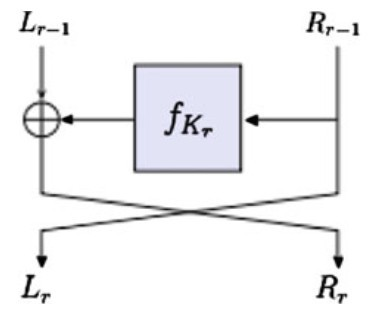
\includegraphics[width=200pt]{Feistel.jpg}
\label{des_feistel}
\end{figure}

\begin{figure}
\centering
\caption{f函数}
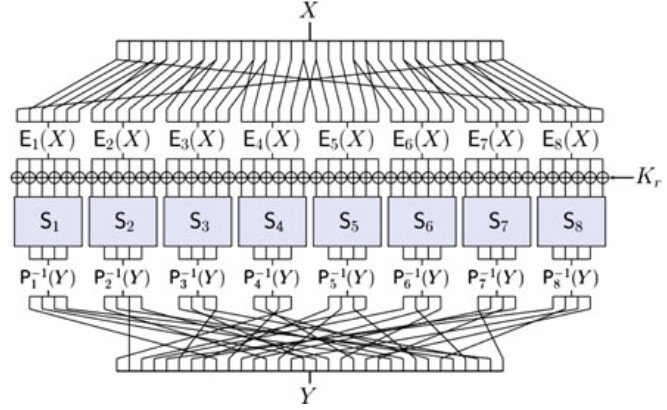
\includegraphics[width=400pt]{des_f_function.jpg}
\label{des_f_function}
\end{figure}


\subsubsection{对DES的第16轮攻击}
假设在第16轮开始的时候,$R_{15}$的一些比特翻转,那么由图\ref{des_feistel}可得$R_{16}$和$R_{16}^*$的差分满足等式:

\begin{equation}
\label{eq:3_1}
\Delta R_{16} = f_{K_{16}} \oplus f_{K_{16}}(L_{16}^*)
\end{equation}

由图\ref{des_f_function}可知,f函数中的S盒独立进行计算,所以上式可以转换成8个等式,其中$(1 \leq i \leq 8)$:

\begin{equation}
\label{eq:3_2}
P_i^{-1}(\Delta R_{16}) = S_i(E_i(L_{16}) \oplus K_{16,i}) \oplus S_i(E_i(L_{16}^*) \oplus K_{16,i})
\end{equation}

因此攻击者可以通过验证$K_{16,i}$的所有可能值${0,1}^6$,排除不满足等式\ref{eq:3_2}的值,最终得到密钥。值得注意的是本攻击只适用于只影响$R_{15}$的故障故障类型,并且$R_{15}$被故障翻转的比特数越多,有效的S盒也越多(即受影响的S盒),所需要的密文对$(C,C^*)$则越少。

\subsubsection{对DES的第15轮攻击}
假设在第15轮开始的时候,在$R_{14}$上注入单比特故障,令$R_{14}^*=R_{14} \oplus \epsilon$,由图\ref{des_error_propagation_15_round}可得:

\begin{equation}
\label{eq:3_3}
\Delta R_{16} = f_{K_{16}}(L_{16}) \oplus f_{K_{16}}(L_{16}^*) \oplus \epsilon
\end{equation}

在上式中$K_{16}$不是唯一的未知参数,因此接下来需要确定或者缩小$\epsilon$的取值范围。利用式\ref{eq:3_4}可以推出第15轮的有效S盒,进而可以根据S盒的有效情况缩小$\epsilon$的取值范围,如果两个S盒有效,则$\epsilon$的值有2种可能,因为由图\ref{des_f_function}可知每对S盒最多共享两个输入比特;同理如果只有一个S盒有效,$\epsilon$的值也有两种可能,因为有效S盒的6个输入比特中与相邻S盒无关的只有2个比特。

\begin{equation}
\label{eq:3_4}
\Delta L_{16} = f_{K_{15}}(R_{14}) \oplus f_{K_{15}}(R_{14}) \oplus \epsilon
\end{equation}

\begin{figure}
\centering
\caption{15轮的错误扩散}
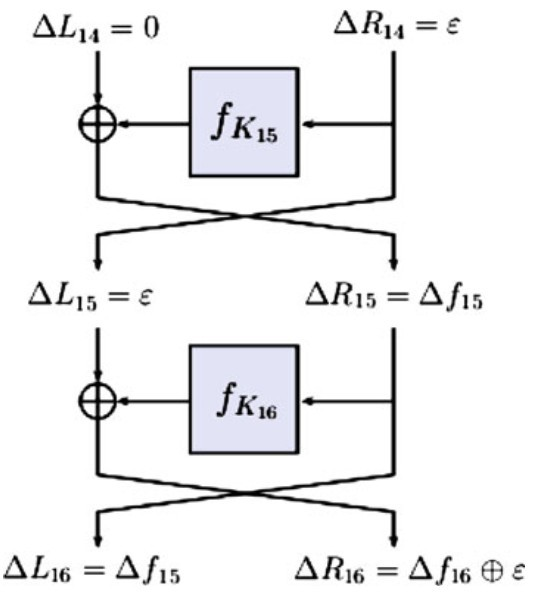
\includegraphics[width=200pt]{des_15_round_propagation.jpg}
\label{des_error_propagation_15_round}
\end{figure}

一旦$\epsilon$的范围确定,就可以用等式\ref{eq:3_3}推出8等式\ref{eq:3_5}(其中$1 \leq i \leq 8$),进而筛选出密钥$K_{16}$。

\begin{equation}
\label{eq:3_5}
P_i^{-1}(\Delta R_{16} \oplus \epsilon) = S_i(E_i(L_{16}) \oplus K_{16,i}) \oplus S_i(E_i(L_{16}^*) \oplus K_{16,i})
\end{equation}

与上一节的攻击相比,本攻击为单比特故障模型(或者只有很少的几个比特故障),因为需要缩小$\epsilon$的取值范围。又因为在第16轮错误被扩散到多个S盒,所以$K_{16}$的筛选效率并不比第16轮的攻击低多少。

\subsubsection{对DES的中间轮攻击}
针对中间轮DFA的基本原理是式\ref{eq:3_6}。在前面的攻击中,攻击者利用$\Delta L_{15}$的值已知或者候选值很少的情况推出密钥。事实上,实施攻击并不一定要恢复出$\Delta L_{15}$的值,只要$\Delta L_{15}$的统计分布明显偏置,就能构造错误密钥区分器,进而筛选出密钥。

\begin{equation}
\label{eq:3_6}
\Delta R_{16} = f_{K_{16}}(L_{16}) \oplus f_{K_{16}}(L_{16}^*) \oplus \Delta L_{15}
\end{equation}

$\Delta L_{15}$的统计分布跟故障翻转的平均比特数和故障位置到$L_{15}$的路径经过的f函数次数有关。例如,如果在$L_{13}$导入故障$\epsilon$,那么$\Delta L_{15} = \Delta L_{13} = \epsilon$。如果$\epsilon$的汉明重量很小,那么$\Delta L_{15}$的分布将严重偏离均匀分布。更一般的,由图\ref{des_error_propagation}可知,$L_{12}$到$L_{15}$仅经过f函数1次,$L_{11}$到$L_{15}$经过2次。由于DES的f函数的扩散不是很快,在$L_{12}$和$L_{11}$注入的故障将导致$\Delta L_{15}$的分布明显偏离。

\begin{figure}
\centering
\caption{$L_{11}$和$L_{12}$到$L_{15}$的错误扩散路径}
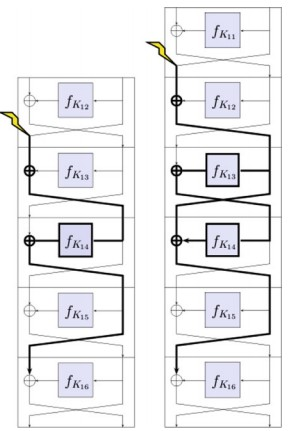
\includegraphics[width=200pt]{des_error_propagation.jpg}
\label{des_error_propagation}
\end{figure}

定义$g_i((C,C^*),k)=S_i(E_i(L_{16}) \oplus k) \oplus S_i(E_i(L_{16}^*) \oplus k) \oplus P_i^{-1}(\Delta L_{15})$为预测$P_i^{-1}(\Delta L_{15})$的函数,$p_i(\delta)$为$P_i^{-1}(\Delta L_{15}) = \delta$的概率,则由分组密码分析中著名的错误密钥假设可得

\[
  Pr[g_i((C, C^*), k) = \delta] = \left\{ 
  \begin{array}{l l}
    p_i(\delta) & \quad if \quad k = K_{16,i} \\
    \frac{1}{16} & \quad otherwise \\
  \end{array} \right.
\]

因为$p_i(\delta)$明显偏离均匀分布,所以可以用数理统计中经典的极大似然估计或者用欧氏距离估计(SEI)来区分出正确密钥$K_{16,i}$,对应的区分器分别为

\[
d(k)=\sum_{n=1}^{N}log(p_i(g_i(C_n,C_n^*, k)))
\]

和

\[
d(k) = \sum_{\delta \in \{0,4\}^4}( \frac{\{\#n;g_i(C_n,C_n^*,k) = \delta\}}{N} - \frac{1}{16})^2
\]

表\ref{tab:3_1}为模拟实验的攻击结果,由表可知本节的攻击对于第11轮和第12轮注入的故障所需的故障数很少,对于第10轮和第9轮注入的故障所需的故障数相对较多,所以为了抵抗本节的DFA,相应的DES算法至少保护最后6轮。

\begin{table}
\centering
\begin{tabular}{*{6}{c}}
注入轮 & 区分器 & 比特故障 &  & 字节故障  &   \\
\cline{3-3} \cline{5-5}
 & & 选择位置 & 随机位置 & 选择位置  & 随机位置  \\
\hline
12 & 极大似然 & 7 & 11 & 9 & 17 \\
   & 欧氏距离 & 14 & 12 & 17 & 21 \\
11 & 极大似然 & 11 & 44 & 210 & 460 \\
   & 欧氏距离 & 30 & 71 & 500 & 820 \\
10 & 极大似然 & 290 & 1500 & 13400 & 18500 \\
   & 欧氏距离 & 940 & 2700 & 26400 & 23400 \\
9  & 极大似然 & $3.4*10^5$ & $2.2 \times 10^7$ & $>10^8$ & $>10^8$ \\
   & 欧氏距离 & $1.4 \times 10^6$ & $>10^8$ & $>10^8$ & $>10^8$ \\
\end{tabular}
\caption{针对DES中间轮的攻击结果}
\label{tab:3_1}
\end{table}

\subsubsection{AES故障攻击}

自从2000年被选为Advanced Encryption Standard(AES),Rijndael得到了越来越多的应用,出现了大量关于AES故障攻击的研究。本节选取几种最为典型的针对AES的故障攻击加以描述。

由AES的密钥生成算法已知最后一轮的轮密钥,攻击者可以恢复128比特AES的主密钥。对于192,256比特AES需要知道倒数两轮的轮密钥才可以完整恢复主密钥。以下的几种故障攻击方法都专注于讨论如何恢复最后一轮子密钥。对于192,256比特AES,可以先使用同样方法恢复最后一轮子密钥,然后将故障注入轮数提前一轮,所得正确错误密文用最后一轮子密钥解密一轮,将得出的中间状态值视为当前情况的正确错误密文对,使用和恢复最后一轮轮密钥类似方法可以恢复出倒数第二轮子密钥,形成完整的攻击。

下面描述的第一种攻击采用随机单字节故障模型,故障注入在倒数第二轮且在列置换操作之前的任一字节。此时攻击的目标状态为倒数第二轮的列置换之前,经过一轮的故障传播在该目标状态的每一列有且仅有一个字节的正确错误状态的差分值非零。攻击者猜测最后一轮子密钥的四字节,对正确和错误密文分别进行部分解密,根据目标状态相应列是否符合前句所述的模式即可排除错误的密钥的猜测。每组这样的猜测可以用于确定相关四字节的子密钥,因此通过四组这样的猜测就可以最后一轮子密钥的恢复。已有的模拟实验显示通过2组正确错误密文对攻击者能以92\%的概率唯一的确定最后一轮的轮密钥。

第二种攻击仍然采用随机单字节故障模型,但是故障注入的轮数相对第一种攻击提前一轮。此时在倒数第二轮的列置换之前的状态的每个字节的差分值均不为0,正确错误的中间状态可用正确错误密文对和最后一轮子密钥标示。同第一种方法类似,攻击者猜测最后一轮子密钥的四字节并做部分解密检测在目标状态的每个字节的差分值是否都非0,若满足,则保留为候选密钥。对于子密钥$K^{r}_{0},K^{r}_{7},K^{r}_{10},K^{r}_{13}$,满足的等式如~。模拟实验显示约1000对密文对可以将密钥空间降低为$2^{40}$。

\begin{equation}
MC^{-1}|_{0}(SB^{-1}(C_{0}\oplus K^{r}_{0})) \oplus MC^{-1}|_{0}(SB^{-1}(C'_{0} \oplus K^{r}_{0} ) \neq 0

MC^{-1}|_{1}(SB^{-1}(C_{13}\oplus K^{r}_{13})) \oplus MC^{-1}|_{1}(SB^{-1}(C'_{13} \oplus K^{r}_{13} ) \neq 0

MC^{-1}|_{2}(SB^{-1}(C_{10}\oplus K^{r}_{10})) \oplus MC^{-1}|_{2}(SB^{-1}(C'_{10} \oplus K^{r}_{10} ) \neq 0

MC^{-1}|_{3}(SB^{-1}(C_{7}\oplus K^{r}_{7})) \oplus MC^{-1}|_{3}(SB^{-1}(C'_{7} \oplus K^{r}_{7} ) \neq 0
\end{equation}

上述攻击的故障模型比较简洁,第三种攻击采用更为复杂的故障模型。可以观察到,当故障发生在倒数第三轮的输入状态的某一对角线时,本轮结束时的状态的差分值全部集中在一列上。在倒数第二轮的列置换之前每一列仍然只有一个字节的差分值不为0.若故障注入在第一对角线,经过推导可以的得出如下等式。

\begin{equation}
SB^{-1}(C_{0}\oplus K^{r}_{0}) \oplus SB^{-1}(C'_{0} \oplus K^{r}_{0} ) = 2(SB^{-1}(C_{13}\oplus K^{r}_{13}) \oplus SB^{-1}(C'_{13} \oplus K^{r}_{13} ) )

SB^{-1}(C_{10}\oplus K^{r}_{10}) \oplus SB^{-1}(C'_{10} \oplus K^{r}_{10} ) = SB^{-1}(C_{13}\oplus K^{r}_{13}) \oplus SB^{-1}(C'_{13} \oplus K^{r}_{13} )

SB^{-1}(C_{7}\oplus K^{r}_{7}) \oplus SB^{-1}(C'_{7} \oplus K^{r}_{7} ) = 3(SB^{-1}(C_{13}\oplus K^{r}_{13}) \oplus SB^{-1}(C'_{13} \oplus K^{r}_{13} ) )
\end{equation}

攻击者首先猜测$K^{r}_{0}$和$K^{r}_{13}$,如果猜测值满足上述第一个等式则保留为候选密钥字节,否则为错误密钥。结合$K^{r}_{13}$的候选值和$K^{r}_{10}$的所有可能值并测试其是否满足上述第二个等式可以进一步减少密钥空间,随后将同样的方法运用到第三个等式,通过以上三组操作$(K^{r}_{0}, K^{r}_{7}, K^{r}_{10}, K^{r}_{13})$的可能值的数量平均为$2^{8} = 256$个。

对于目标状态的其他三列也有类似的结果,这样最后可以将最后一轮轮密钥的密钥空间降低到$(2^{8})^{4}=2^{32}$。上述讨论中故障所处的对角线已知,如果故障发生的对角线未知,需要猜测所有可能四种情况,密钥空间是已知对角线情况的4倍。

上述攻击可以被扩展到在倒数第三轮的输入状态上至多三个对角线上的值受影响的故障模型。此时可以列出类似上述所示等式组,具体的等式会稍微比较复杂,如果没有发生故障的对角线已知,等式组成的密钥区分器可以将猜测的4字节的密钥空间降低到$2^{24}$。在这样的故障模型下,使用四对正确错误密文对,最后一轮轮密钥可以以很大的概率确定。

\subsubsection{RSA故障攻击}
\subsubsection{ECC故障攻击}
\subsubsection{其他算法包括轻量级算法的故障分析}
\subsubsection{流密码和哈希函数的故障攻击简介}

\subsection{故障攻击实验环境:包括已有的故障攻击实施工具和攻击过程,如电压和时钟Glitch,激光和电磁辐射等}
故障注入是一次实际的完整的故障攻击的第一步,故障注入的结果直接决定了故障模型、相应的攻击方法和之后故障分析的复杂度如何。故障分析采用的故障模型必须能够和某种故障注入方式相吻合。故障注入的方式多种多样,原理、攻击平台、攻击效果各不相同,完成攻击所需要的造价也有很大差异。按照其作用效果可分为全局型的故障注入和局部型的故障注入,瞬时的故障和永久的故障。按照攻击前对目标芯片的处理程度可分为侵入式攻击和非侵入式攻击。本章将逐一列举几种常见的且比较有效的攻击方式和在这方面的一些攻击结果。由于故障注入的多样性,以下的小节中将以特定的攻击实验来组织描述,试图达到窥一斑而知全豹的效果。

\subsubsection{电压和时钟的故障实验环境和注入结果}

电压和时钟攻击在芯片的电压或时钟输入管脚提供不正常的输入来影响电路运行使之出错。不正常的输入可以使过高或是过低的电压,电压或是时钟上的毛刺等。电压和时钟的攻击是一种全局性的注入方式,故障影响整个芯片电路,故障注入可以再时间上有比较精确的控制但是无法对某一些运算单元单独注入故障。同时完成电压和时钟注入所需的成本较低,因此的到了广泛的应用和研究。
在CMOS电路中,每个门电路上都存在着电容因此都会有传播延时,在门电路的输入端的变化需要一段时间才会产生相应输出。传播延时的长短是由好多因素共同决定的。其中最主要的决定因素是门电路所做的运算,例如,在与门中,一个输入端为0的话,无论另一个输入端如何变化,结果恒为0;而或门就没有这样的特性。输入信号的形状也会影响传播延时,信号经过长的连线后会有比较平滑的边缘,而有良好缓存只经过短的线路的信号有比较陡峭的边缘,连线的长短也间接地影响了传播延时。其他会影响传播延时的因素有连线之间的耦合,一些门电路的不确定的响应时间和电路中产生的毛刺等。因而必须在等电路输出稳定之后才可以获得需要的结果。
在时序电路中,时钟信号并行的与所有组合电路发生关联,这意味着当时钟信号的上升边缘来临时所有门电路都已完成结果的稳定输出。这样最长的传播路径就决定了电路的最大时钟频率。这个最大的传播延时就叫做启动时间。如果出于一些原因使时钟间隔变短或启动时间变长,时钟间隔小于启动时间,错误就有可能发生。
实验结果显示传播延时会随着供电电压的变低而逐步变长,在实验中使用的电路的极限供电电压0.4V下,输出结果经过很长时间都没有收敛。如果该传播延时没有影响在最长传播路径,则没有故障;否则,时钟上升沿在输出信号变化时采样,就有一定概率出错或是逻辑门电路输出值为错误结果就会导致故障。实验结果显示温度也会对传播延时产生影响但是影响较小。

本节中讨论的实验是针对ASIC实现的AES。故障注入设备包括与智能卡读卡器,稳压电源和一个任意波形的信号发生器。这样就可以为智能卡提供各种不同的电压和时钟信号。实验中使用的智能卡是130nm的ASIC,额定供电电压是1.2V。故障注入过程选取的智能卡能正常工作同时又有一定出错概率的电压范围为775-825mV,电压变化的步长为0.5mV,共100组实验。每组实验包括20,000次故障注入,在每组实验中密钥被设置为固定值,明文可以发生变化。实验显示通过降低供电电压可以产生一般的故障分析所需要的单个字节的故障模型。在实验中可观察到随着电压的降低发生故障的可能性逐步增大,但是在所有故障中单字节故障发生的可能性有所不同,单字节故障随电压变化基本符合钟形分布,在800mV的时候概率最大,约占所有故障的30\%。同时发生的单字节故障的轮数和所在的位置并不是随机分布的。在刚开始发生故障的电压处,单比特故障较多,但是随着电压逐步降低,多比特故障逐步增多,同时可观察到故障差分值为7,8情况几乎没有,这些结论都与传播延时故障理论相符合。在FPGA上的实验结果与ASIC上的基本相同,因此可以用FPGA来衡量电路抗电压降低的能力。

\subsubsection{电磁故障实验环境和注入结果}

电磁故障注入通过在芯片表面某个点处施加瞬时的强电磁场或是特定的谐波来影响该点处电路的运行,达到故障注入效果。相对于电压和时钟注入,电磁注入可以在控制注入的空间位置,产生局部故障。

现有的研究表明,电磁故障注入不仅可以完成对数字电路的故障注入,同时还可以影响CMOS环形振荡器。CMOS环形振荡器是CMOS电路中很有代表性的电路结构,可以作为时钟信号发生器和真随机数发生器的组成单元。Poucheret等人在内含环形振荡器的电路表面施加1GHz的电场来影响环形振荡器的输出频率。根据观察到的注入结果作者确定了芯片易受谐波电场影响的区域,结合被攻击电路的布局,作者发现注入探针和电路的耦合主要发生在电源接地网络处。进一步的研究表明可以通过这样的故障注入来将基于环形振荡器的真随机数发生器的频率锁定为注入的谐波频率从而控制了真随机数发生器的输出。

以下部分描述Dehbaoui等人对于软硬件实现的AES的瞬时电磁脉冲故障注入结果。实验使用的平台包括控制电脑,电动步进平台,脉冲发生器,磁线圈和测试芯片。脉冲发生器为磁线圈供给电压脉冲,产生的脉冲有5ns的上升和下降时间,脉冲的幅度变化范围为1V~100V,磁线圈的直径为500$/mu m$。软件实现的AES运行在一款8位微处理器上,处理器运行频率为3.57MHz。作者主要研究了在AES最后一轮执行期间的故障注入,结果显示不同的字节会发生常数故障值或是数据相关的故障值。结合执行的汇编代码和注入时间,作者猜测注入导致了部分指令被略过或是发生了改变。另外发生故障的注入占总注入次数的比值随着脉冲电压的升高而增加。硬件实现的AES运行在FPGA上,算法运行频率为100MHz。硬件采用了128比特数据宽度,一轮的AES加密可以在一个时钟周期内完成,AES的轮密钥是在运行时生成的。故障仍是注入在最后一轮,先按照电磁线圈直径将芯片表面划分为30$\times$30的小区间,在每个小区间内执行1000次的故障注入实验。注入结果显示电磁故障注入可以产生单比特和多比特的故障,同时电磁故障是局部的故障注入,和密码较为密切相关的区域发生故障的可能性更高,在不同的位置进行注入所导致的各个字节出错的概率分布也是不同。最容易出故障的位置与最长延时路径单元重叠以及故障注入是数据相关等表明电磁注入可能导致局部数字逻辑供电电压降低,电路传播延时增加违反了电路时间限制从而导致了故障。作者也在原AES电路上实现了检测违反电路时间限制的防护,同时按照与不加防护相同的设置进行了实验。这种防护对于电压故障和时钟故障注入具有比较显著的效果。实验结果显示仅有10\%的故障被检测出,同时还有很多未发生故障但是检测电路有警报的情况,这说明电磁故障注入可以有效的跳过这种防护。

\subsubsection{激光的故障实验环境和注入结果}

光照故障注入是另一类被广泛采用的注入技术,光照故障注入通常需要更昂贵的设备和各专业的操作,但是光照注入技术往往可以达到比较好的空间精度,获得一些全局故障注入技术无法获取的信息。
 
最简单的光照注入技术采用很强的同时精确聚焦的光速来对芯片进行故障注入。对晶体管进行强光照射可在其上的电介质上形成暂时的导电通路,类似于晶体管正确偏置时其上产生的通路。这样就实现以一种精确和可控的方式改变了晶体管的状态。为了达到比较精确的聚焦光束,相机闪光灯产生的光束通过显微镜目镜聚焦到载物台上,在载物台放置了需要注入的芯片。为了防止过度照射对芯片电路的永久性修改攻击者必须仔细的控制显微镜镜头的放大倍数。同时攻击者还需要设计异步电路来控制闪光灯与芯片同步工作。简单光照注入的最大的不足在于自然光无极性,相干性较差,自然光的波长是当前蚀刻工艺门电路的电介质部分的十倍左右,同时显微镜也无法达到精确的聚焦,因而就无法实现对单个逻辑门电路的故障注入。由于闪光灯无法在短时间内产生一系列的闪光,这种技术也无法在设备运行时进行多次的故障注入。

对上述注入技术最直接的改进就是用激光代替闪光灯。故障注入的原理与闪光灯的基本相同,但是激光故障可以更有效在单次照射中注入故障同时也拥有更高的空间精度。同时激光还可以照射芯片背面来进行故障注入。这是通过使用红外激光来实现的,纯的硅晶体对1 $U$m到5 $u$m的光线有50\%的透射。虽然因为硅晶体衬底对激光的散射作用光照的精确度会降低但是背部激光照射可以攻击电路的底层部分。激光的强度必须要精确地加以控制,否则很容易永久性的烧毁芯片。商业的激光注入平台还有激光聚焦镜头,装有精密步进电机的载物平台,激光与芯片的同步电路等来完成完整的高精度的故障注入。激光注入无法达到亚波长的精度,因而其影响的门电路的数目与激光波长与蚀刻工艺有关。激光需要较短的时间来重启动所以可以被用来在芯片运行时进行多次故障注入。多故障注入将在下一节进行更为详尽的讨论。

激光注入具有很高的时间和空间精度,可以非常好的实现对未加防护密码芯片的故障注入。下面的介绍的实验比较了激光注入在带防护有不带防护电路的故障注入结果获得激光注入的一些特性。该实验的攻击对象为一款完成512比特蒙特玛丽模乘的协处理器。协处理器拥有组合运算单元,移位寄存器,控制电路,IO寄存器等模块。带防护的电路中实现了简单的奇偶校验和双轨逻辑。每32位寄存器或锁存器都有一位校验,组合运算单元也双轨逻辑和相应错误检测方案。该防护电路在电路效率和安全级别方面做了折中,寄存器校验位可以检测奇数位的比特出错。实验采用了完善的故障注入平台将未加防护和加防护电路划分成多个矩形小区间,在每个区间又在每个运行的时间段内进行了5次激光故障注入实验,对两种电路的故障注入次数分别为1350和2250。注入中运算时钟采用相同的输入参数并且激光的强度恒定。实验结果显示所有的故障注入都导致了电路的非正常运行。在加防护电路中产生了6次未被检测的故障注入,这意味着攻击者可以利用激光实现对类似防护电路的故障注入。这6次故障都集中于同一个矩形小区间,具体的原因还需要进一步的实验和理论检测。实验中还观察到对于带防护电路产生的故障不是确定性的,虽然激光针对的区域较小,但对单个区域单次的故障注入可能导致多个校验位的出错,这与一些理论分析中所假设的单比特故障有很大不同。

另外的实验研究了不同类型电路单元在激光注入下的不同响应特性,为激光注入产生故障的成因和设计抗激光注入的单元级电路提供了参考。
\subsubsection{多点故障注入的实验环境和实验结果}
\subsection{抗故障攻击的防御方法}
故障攻击从1997年提出到现在,发展迅速,对许多经典加密算法的实现提出了更高的要求,比如只需要一个故障,就能在极短的时间内恢复出AES-128和RSA-CRT的全部密钥。因此对于一些安全性要求较高的设备,比如交通卡、SIM卡来说,设计针对性的防御方法变得至关重要。目前已经有很多文章提出了相应的防御方法,基本原理都是通过增加冗余计算,从而防止攻击者获得错误密文或者有效的错误密文,根据原理可以将这些防御方法大致分为检测和干扰两个类别,本章将分别介绍这两类防御方法的原理、目的、适用范围及不足。
\subsubsection{基于检测的防御方法}
检测的主要原理是在算法的运行过程中受到干扰时,中断算法的运行,这样就可以防止输出错误密文,从而防止故障攻击。有很多方法利用错误检测代码来检测是否有故障注入,但是文章「37」表明这些方法并没有比简单的重复算法更有效。同时由于各种加密算法都需要采用掩码机制来防御功耗攻击等旁路攻击方法,在些基础上实现错误检测并不容易。基于上述原因现实中采用更多的是加密算法的重复计算,这也是本节介绍的重点。
重复计算可以分为三大类:完全重复计算、加密解密计算和部分重复计算。完全重复计算是指加密明文两次,检测得到的密文是否相同。可以由两种方式实现完全重复计算,一种是用同一个电路先后计算两次,这会使算法的执行时间加倍;另一种是用两个相同的电路同时计算两次,这会增加实现算法的电路空间面积,在不增加计算时间的同时,还能防御注入的永久性故障。加密解密计算是指先对明文执行加密算法得到密文,然后对密文进行解密,检测解密得到的明文与原明文是否相同。部分重复计算是指对明文进行一次完全的加密和重复后几轮的加密操作,检测得到的密文是否相同,这种方法之所以有效,是因为大部分DFA都需要在算法的后面几轮注入故障。如果攻击者可以对解密得到的密文,那么部分重复计算的方法将失效,因为攻击者可以利用正确密文和错误密文对$(C,C^*)$进行解密得到明文对$(P,P^*)$,然后可以对$(P,P^*)$实施攻击。同时这种方法对于安全故障攻击无效,因为攻击者可以根据是否输出密文来判断故障是否有效,针对安全故障攻击比较好的方法是对中间数据进行冗余检测,比如引入循环冗余码(CRC)。
一般对于a和b的比较操作会泄露a和b的组合信息,特别是异或信息,因为比较通常通过减或者异或实现。如果通过异或实现,将直接泄露a和b的异或信息;如果通过减实现,a-b等于a异或b的根据大于35%。因此攻击可以先通过功耗和故障的组合攻击实施攻击,比如对于完全重复计算的防御方法来说,攻击者可以先利用功耗攻击获取正确密文和错误密文对的异或信息$C \oplus C^*$,再通过DFA实施攻击。同时文章「28」「31」表明,比较操作很容易被注入故障绕过,所以还需要基于干扰的防御方法来保护这种脆弱的操作。

\subsubsection{基于干扰的防御方法}
干扰的主要原理是扩大故障导致的逻辑影响,从而改变算法的扩散模型,使输出的错误密文很难被攻击者利用。图\ref{infection_countermeasure}以AES算法为例,用上一节基于检测的方法同时进行两个加密运算,假设攻击者在某一轮的状态S上注入故障,那么差分$S \oplus S^'$通过扩散函数$D()$将被扩散到整个状态,然后再进入下一轮进行运算。目前已经有很多基于以上原理的干扰方案,比如文章「28」和「20」分别提出了AES上的干扰方案,但由于这些方案都是采用固定的扩散函数,所以存在缺陷。比如就AES的最后一轮的字节故障模型来说,攻击者可以根据故障模型提前计算$2^8-1=255$种可能的故障类型,因为扩散函数是固定的,所以可以计算出经过函数$D()$扩展后的状态$\Gamma$的255种可能情况,最后每次猜测两个字节的密钥从明文反推出一个字节的差分值,通过比较该差分值是否在$\Gamma$的取值范围内,判断猜测是否正确,从而筛选出部分密钥。

\begin{figure}
\centering
\caption{基于干扰的防御原理}
\includegraphics[width=200pt]{infection_countermeasure.jpg}
\label{infection_countermeasure}
\end{figure}

\subsubsection{掩码防护方案}
\subsubsection{抗故障攻击的电路单元}
\end{CJK}


\end{document}